
\documentclass[10pt]{article}
\usepackage{graphicx}
\usepackage{subcaption}
\usepackage{hyperref}
\usepackage[ngerman]{babel}
\usepackage{siunitx}
\sisetup{locale=DE, per-mode=symbol  % whether it should print "/" or "^-1"
}

\usepackage[margin=2cm]{geometry}
\usepackage[utf8]{inputenc}
\usepackage{multicol}
\usepackage{nicefrac}
\usepackage{todonotes}
\usepackage{amsmath}
\usepackage{csquotes}
\usepackage{amssymb}
\DeclareMathOperator{\sign}{sign}
\usepackage{wrapfig}
% \usepackage{pdflscape}
% \usepackage{pdfpages}
% \usepackage{epstopdf}
% \epstopdfDeclareGraphicsRule{.tiff}{png}{.png}{convert -density 180 #1 \OutputFile}
% \AppendGraphicsExtensions{.tiff}


\author{Felix Ganz\thanks{Projektgruppe 03 in der Lehrveranstaltung \glqq{}Autonomes Fahren\grqq\ an der \emph{TUHH} und der \emph{UHH}}\and Nico Albers\footnotemark[1] \and Tim Hansen\footnotemark[1]\and Timo Kias\footnotemark[1]}
\title{Abgabe 2: \emph{Abstandsregler}}

%\setcounter{tocdepth}{1}
\begin{document}

\maketitle
%\tableofcontents

\section{Bilderkennung}
    Zur Erkennung des vorausfahrenden Fahrzeugs haben wir zunächst gängige in OpenCV implementierte Bilderkennungsalgorithmen genutzt, um ein Rechteck um das gefundene
    Fahrzeug zu legen.
    Diese Algorithmen haben in unseren Experimenten nicht zufriedenstellend gearbeitet, insbesondere in Kurvenfahrten zeigte sich eine hohe Fehleranfälligkeit, wir haben deshalb den im Folgenden beschriebenen selbst entwickelten Ansatz zur Erkennung verfolgt.

    Anstelle der Erkennung des gesamten Fahrzeugs im Bild versuchten wir, markante Merkmale des vorausfahrenden Autos zu identifizieren und nur diese zu erkennen.
    Unter der Annahme, dass das zu folgende Auto von gleicher Bauart wie unser eigenes Auto ist, haben wir die rot eingefärbten Federn der Hinterradaufhängung als passendes Merkmal hierzu identifiziert.
    Dies ist keine zu große Einschränkung, diese Methode kann für einen allgemeineren Ansatz (wie ein vorausfahrendes Fahrzeug mit anderem Aufbau) durch Hinzufügen erkennbarer Merkmale entsprechend adaptiert werden.
    Da die Radaufhängung grundsätzlich über das Farbspektrum der entsprechenden Pixel identifizierbar ist und prinzipiell formunabhängig ist, hielten wir diesen Ansatz für vielversprechend.
    Ein weiterer Vorteil dieser Idee ist, dass wir zwei Federn identifizieren können, was später im Zusammenhang mit der Abstandsreglung ein entscheidender Faktor sei wird.

    Für die Identifikation der roten Federn haben wir das Farbspektrum der Pixel untersucht und dieses nach ihren HSV-Koordinaten\footnote{Hue, Saturation und Value} mit Hilfe einer Maske gefiltert\todo{?}, vergleiche Abbildung~\ref{fig:cars}.
    Dies bietet eine gute Möglichkeit passende Ober- und Untergrenzen möglicher Koordinaten zu definieren, mit der wir die bereits erwähnte Maske bilden um die Pixel nach ihrem Farbspektrum zu filtern.
    Über die $H$ Koordinate kann dabei der Farbton rot relativ direkt benannt werden.
    Über die $S$- und $V$-Koordinaten konnten wir Farbintensität und Helligkeit einstellen.
    Mit der HSV-Maske können wir das Bild in eine binäre Darstellung überführen, in der Pixel mit HSV-Werten innerhalb der definierten Grenzen als weiße Pixel und Pixel mit Werten außerhalb der Grenzen als schwarze Pixel dargestellt werden.
    Mit dieser klaren Abgrenzung von roten zu andersfarbigen Pixeln, haben wir eine Reihe von Regeln erstellt, mit der gefundene rote (nun weiße) Bereiche als Federn identifiziert werden konnten.
    Nachdem zwei passende rote Felder gefunden wurden, haben wir jeweils Hüllkreise mit minimalem Radius um diese gezogen, sodass alle identifizierten Punkte innerhalb dieser Hülle liegen.
    Mit der hiermit konkretisierten Geometrie der gefundenen Federn waren wir in der Lage zunächst die Mittelpunkte und daraufhin den Abstand zwischen diesen in Pixelkoordinaten zu identifizieren.
    \todo[inline]{TODO:\@ angaben weiterer Verfeinerungen der Grundidee Vorverarbeitung des Kamerabildes eventuell  einige der Regeln}

    \begin{figure}[htbp]
        \centering
        \begin{subfigure}[b]{0.4\textwidth}
            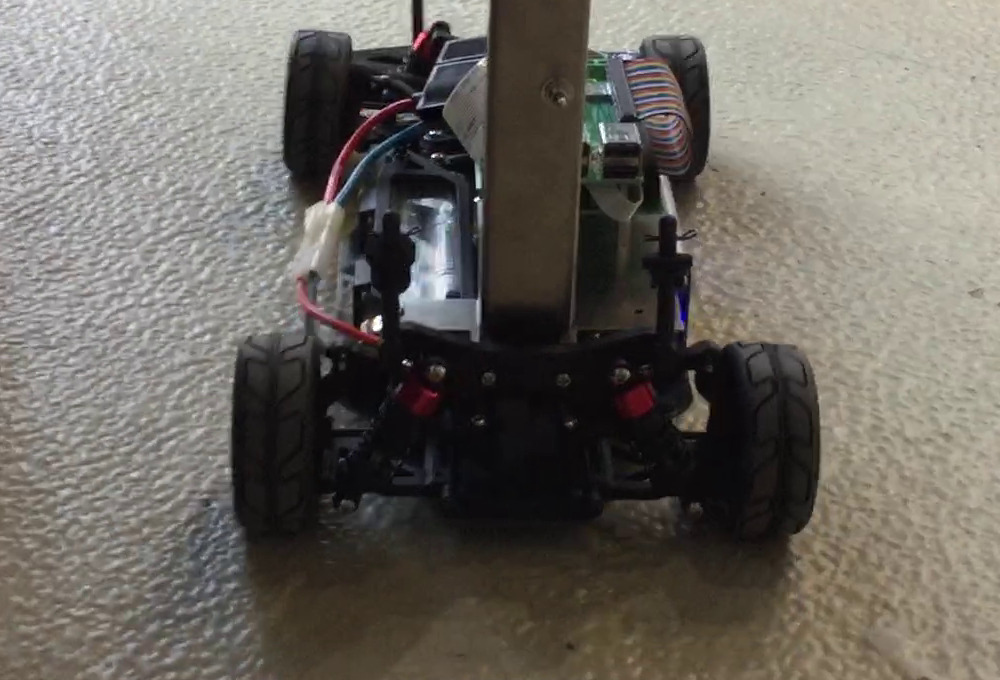
\includegraphics[width=\textwidth]{car}
            \caption{Bild des Autos}\label{fig:car}
        \end{subfigure}~\begin{subfigure}[b]{0.4\textwidth}
            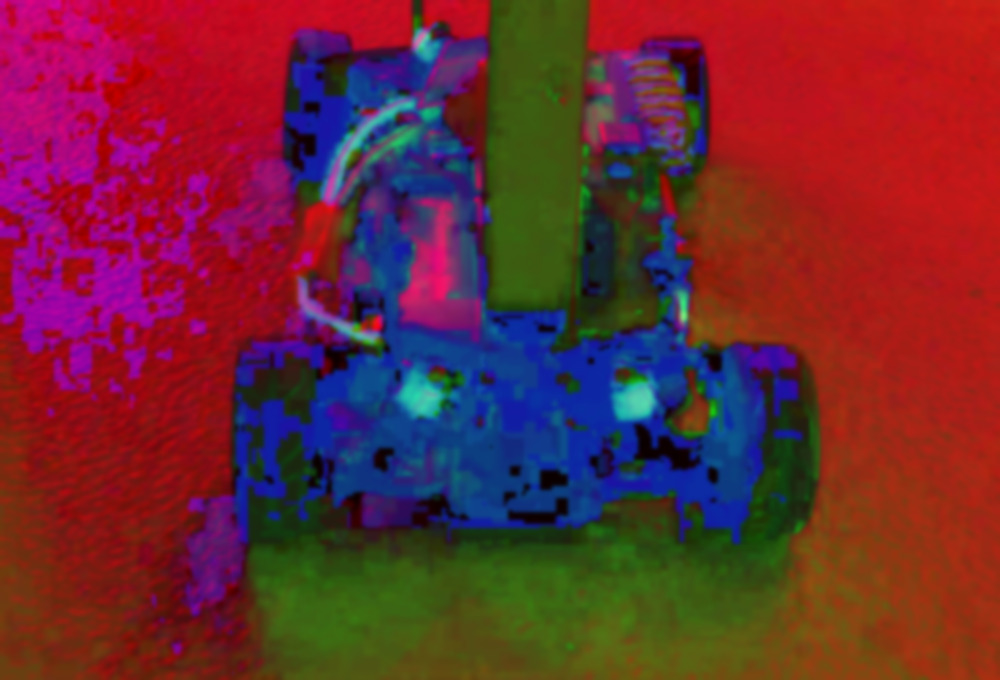
\includegraphics[width=\textwidth]{car_hsv}
            \caption{HSV-gefiltertes Bild}\label{fig:car_hcsv}
        \end{subfigure}
        \caption{Bild und gefiltertes Bild des Autos}\label{fig:cars}
    \end{figure}


    \subsection{Robustheit und Performance}\label{sub:robustheit_und_performance}
        Für die Bilderkennung der beiden roten Punkte am Auto haben wir die Robustheit und Performance optimiert.
        Problematisch hierbei ist die geringe Größe der beiden Federn, die eine hohe Auflösung des zu analysierenden Bildes erfordern und hierdurch die Rechenzeit pro zu analysierendem Frame erhöhen.
        Als praktikable Lösung hat sich herausgestellt, das Bild in einer Größe von $748\times 572\,\text{px}$ aufzunehmen, die seitlichen Ränder und das obere Drittel zu entfernen und dann auf $60\%$ der eingelesenen Auflösung zu skalieren.
        Hilfreich an diesem Vorgehen ist die bessere Erhaltung der Farbwerte bei dem Skalieren als dies beim Auslesen der Kamera mit niedriger Auflösung passiert.
        Es war letztendlich möglich, die Bilderkennung mit \SI{15}{\hertz} und somit einer ausreichend hohen Frequenz für die Regelung durchzuführen.

        Um fehlerhaft erkannte Punkte (False Positives) auszuschließen und die Robustheit zu erhöhen, wenden wir logische Regeln an.
        Diese sorgen dafür, dass erkannte rote Punkte anhand ihrer Grösse und Position ausgeschlossen werden.
        Weiter lässt sich auch bei nur einem im Bildausschnitt erkannten Punkt die Kenntnis des zweiten Punkts sicherstellen.

        Diese Methode hat noch einige Problematiken.
        So arbeitet die Erkennung bei keinem erkannten Punkt (wenn das Auto beispielsweise \glqq{}aus dem Bild fährt\grqq{}) nicht mehr einwandfrei und fehlerhaft.
        Wir koennen zum aktuellen Zeitpunkt diese Punkte nicht wiedererkennen, ohne das zu verfolgende Auto wieder in die Mitte des Bildes zu stellen.
        % subsection robustheit_und_performance (end)



\section{Abstandsregelung}\label{sec:Abstandsreglung}
    Im Folgenden stellen wir unsere Überlegungen für das Problem der Abstandsregelung dar.
    Bei der Betrachtung dieser Regelungsaufgabe wurde schnell klar, dass das grundlegende Problem darin besteht, dass unsere Bilderkennung Information in Pixelkoordinaten eines zweidimensionalen Raums liefert.
    Nach einiger Recherche zu möglichen Rücktransformationen von zweidimensionalen Pixelkoordinaten zu dreidimensionalen Weltkoordinaten war die Problematik dieser Aufgabenstellung umso deutlicher.
    Ohne zusätzliche Informationen darüber was in dem Bild zu sehen ist, sind direkte analytische Lösungen nicht vorhanden und auch mit Informationen über bekannte Geometrien im Bild sind weitere Annahmen nötig, um auf eine eindeutige Tiefe in Weltkoordinaten Rückschlüsse zu führen.
    Mit der Annahme, dass das Zielobjekt auf einer ebenen Fläche fährt und das die identifizierte Punkte parallel zu dieser Fläche liegen, ist eine Rückrechnung der Pixelkoordinaten in Weltkoordinaten mit Hilfe der identifizierten Federn aus der Bilderkennung und deren Abstand zueinander zumindest für die Pixel möglich, die das Auto darstellen.
    Damit lässt sich auch der Abstand des Hecks zu der Kamera des folgenden Autos bestimmen.
    Die Überlegung hierzu beruht auf dem in Abbildung~\ref{fig:reifenradius} dargestellten Schema.

    Bei bekannter Größe des Objekts $H$ in Weltkoordinaten und $h$ in Bildkoordinaten sowie ermitteltem Fokus $f$ kann der Abstand $z$ durch \[
    z = \frac{fh}{H}
    \] berechnet werden.
    Unter Verwendung dieses einfachen Zusammenhangs könnte man nun aus den ermittelten Abständen der Federn aus der Bilderkennung und bekanntem Abstand der Federn am realen Auto den Abstand von Kamera zu vorausfahrendem Auto ermitteln und dann über eine weitere Transformation von Kamerakoordinatensystem zu einem autofesten Koordinatensystem den Abstand zwischen Front und Heck der Fahrzeuge ermitteln.

    \begin{figure}[hbtp]
        \centering
        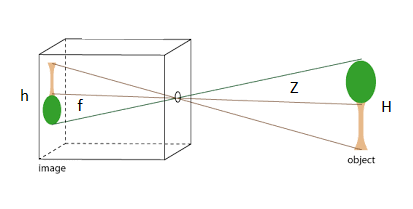
\includegraphics[width=0.45\textwidth]{Pinholeobject_label}
        \caption{Schematische Darstellung der Tiefeninformation bei bekannter Geometrie}\label{fig:reifenradius}
    \end{figure}
    Stattdessen haben wir uns für eine Lösung entschieden, die auch als \textit{vision based control} bekannt ist.
    Bei dieser Art der Abstandsregelung haben wir auf die Transformation von Pixelkoordinatensystem zu Weltkoordinatensystem verzichtet und haben die nötigen Berechnung zur Reglung komplett im Pixelkoordinatensystem durchgeführt.
    Unsere Reglerstruktur besteht aus zwei entkoppelten Reglern $C_u$ und $C_{\gamma}$, bei dem der Regler $C_u$ für den Abstand in Tiefenrichtung und der Regler $C_{\gamma}$ für den Abstand in Breitenrichtung verantwortlich ist, beide in Bezug auf das Weltkoordinatensystem.
    Da wir jedoch keine Transformation zum Weltkoordinatensystem durchführen, haben wir die Informationen aus der Bilderkennung in entsprechende Fehlergrößen $e_u$ und $e_{\gamma}$ überführt, die dann durch den entsprechenden Regler in eine Motoransteuerung \[u = C_u(e_u)\] und einen Lenkwinkel \[\gamma = C_{\gamma}(e_{\gamma})\] umgerechnet werden.
    Den hierfür benötigten Fehlergrößen liegen folgende Überlegungen zugrunde:
    Für den Abstandsfehler $e_u$ geben wir dem System ein Referenzbild vor, in dem das vorausfahrende Auto im gewünschten Abstand zu dem verfolgenden Auto steht.
    Der über die Bilderkennung ermittelte Abstand der Federn in Pixelkoordinaten dient im folgenden als Referenzgröße $d_{f,r}$.
    Dieser kann bei Bedarf auch \enquote{hart} in Pixelgrößen im System hinterlegt werden.
    Im Laufe der Fahrt wird nun jedes eingehende Bild analysiert und ein aktueller Abstand $d_{f,a}$ mit der Referenzgröße verglichen um den Abstandsfehler \[
    e_u = d_{f,r} -d_{f,a}
    \] zu bilden.
    Vergrößert das vorausfahrende Fahrzeug den Abstand zum Verfolger wird der erkannte Federabstand $ d_{f,a}$ kleiner und die Fehlergröße positiv. Andersherum wird die Fehlergröße negativ wenn sich der erkannte Federabstand vergrößert.
    In diesem Fall nähert sich der Verfolger dem vorausfahrenden Fahrzeug und der Motorinut wird zu Null gesetzt, damit der Verfolger bremst und nicht mit negativer Motoransteuerung rückwärts fährt.
    Für den Lenkfehler $e_{\gamma}$ wird kein Referenzbild benötigt, hier wird zu jedem Zeitpunkt der Mittelpunkt $M=\left[M_x, M_y\right]$ der Verbindungslinie zwischen der in der Bilderkennung ermittelten linken und rechten Feder ermittelt. Daraufhin bilden wir den horizontalen Abstand bezüglich der Bildmittellinie: \[
    e_{\gamma} = x_0 - M_x.
    \]
    Die horizontale Koordinate der Bildmittellinie $x_0$ ist aus der Kamerakalibrierung als zentraler Punkt der Bildebene bekannt.

    In beiden Fällen haben wir den eingehenden Fehler mit dem größten zu erwartenden Fehler skaliert, um den Eingang des Reglers auf den Bereich $\left[-1,1\right]$ zu normieren.
    Durch diesen Schritt vereinfacht sich die Wahl der Reglerparameter.
    Weiter ist eine Abbildung auf den jeweils möglichen Ausgangsbereich für Motoransteuerung und Lenkwinkel besser möglich.
    Als erste Implementierung haben wir die beiden Regler als Proportionalregler ausgelegt.
    Prinzipiell können in dem oben beschriebenen Rahmen aber auch weitere Reglerfunktionen angewendet werden.


\section{Performance und Parameteroptimierung}
    Für diese Abgabe haben wir uns auf die oben beschriebene Reglerstruktur unter Verwendung eines Proportionalreglers beschränkt da wir nach ersten Testläufen mit einem aufgebockten Fahrzeug erkannten, dass unsere Regler zwar das gewünschte Verhalten zeigen aber die Umsetzung nicht in Echtzeit erfolgte.
    Um die Rechenleistung zu erhöhen haben wir das analysierte Bild verkleinert, indem wir nur im Abstand von unseren oben genannten Referenzpunkten gesucht haben.
    Die zugrundeliegende Idee hierbei ist, dass das vorausfahrende Auto sich selbst in Kurven nicht sprunghaft aus unserem Bild entfernt und der betrachtete Ausschnitt mit jedem folgenden Bild in Richtung des Autos versetzt wird.

    Wie in Kapitel~\ref{sec:Abstandsreglung} beschrieben, verwenden wir die beiden Regler $C_u$ und $C_{\gamma}$.
    Der Regler für den Lenkeinschlag $C_{\gamma}(e_{\gamma})$ hat zum Zeitpunkt der Abgabe die interne Struktur
    \[
    C_{\gamma}(e_{\gamma}) = \begin{cases}
        k_{\gamma}e_{\gamma}\gamma_{\max} & |e_{\gamma}| \leq 1 \\
        -\sign (e_{\gamma})\gamma_{\max}  & |e_{\gamma}| > 1
    \end{cases},
    \] mit $k_{\gamma}$ einer proportionalen Verstärkung und $\gamma_{\max}$ dem maximal möglichen Lenkeinschlag des Fahrzeugs.
    Die Fallunterscheidung um den Wert Eins ergibt sich durch eine Skalierung des Fehlerwertes auf einen Toleranzabstand um die Mittellinie des Bildes, welche eingeführt wurde um einem Herausfahren des zu folgenden Fahrzeugs aus dem Bild der aufnehmenden Kamera durch einen maximalen Lenkeinschlag entgegen zu wirken.
    \begin{wrapfigure}{r}{0.5\textwidth}
        \centering
        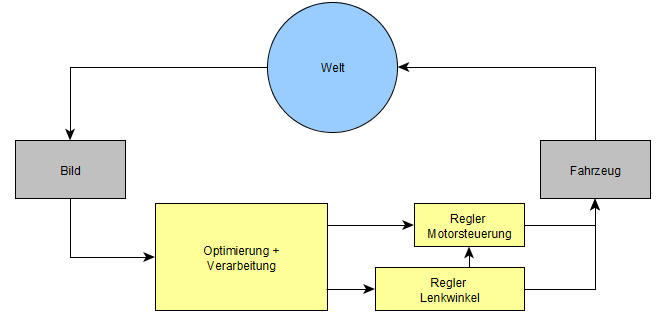
\includegraphics[width=0.48\textwidth]{Autonomes_Fahren_Welt_Regler}
        \caption{Darstellung der Reglerstruktur}\label{fig:struktur}
    \end{wrapfigure}

    Der Regler für den Abstandsregler $C_{u}$ hat zum Zeitpunkt der Abgabe die interne Struktur \[
    C_{u}(e_{u}) = \begin{cases} 0 & e_{u} \leq 0 \\
    \max (fk_{u}e_{u}u_{\max},u_{\min}) &  e_{u} > 0
    \end{cases}
    \]
    mit $f(\gamma) = 1 - \nicefrac{\gamma}{\gamma_{\max}}x$.

    Hierbei sind $k_{u}$ eine proportionale Verstärkung, $\gamma_{\max}$, $u_{\max}$ die jeweils maximalen Ansteuerungen von Motor und Lenkeinschlag und $u_{\min}$ ein minimaler Motoreingang, der nötig ist um die Haftreibung zu überwinden.
    Die zusätzliche Skalierung $f(\gamma)$ modelliert eine Abhängigkeit des erkannten Abstandes der Federn und darüber des vom Regler erzeugten Motoreingangs zum Gierwinkel des vorausfahrenden Fahrzeugs als proportionale Dämpfung des Eingangs $u$.
    Unsere Reglerstruktur ist in Abbildung~\ref{fig:struktur} dargestellt.


\section{Grenzen und Ausblick}
    Die oben beschriebene Methode zur Steuerung des Fahrzeug hat gewisse Grenzen.
    So kann das Fahrzeug nur folgen und sofern das vordere Fahrzeug rückwärts fährt, wird unser Fahrzeug mit diesem kollidieren.

    Zu Beginn haben wir die Regler unabhängig voneinander programmiert.
    Da der Abstand zwischen den getrackten Punkten in einer Kurve allerdings abnimmt, obwohl das führende Fahrzeug sich nicht in diesem Maße vom folgenden Fahrzeug entfernt, haben wir den eingeschlagenen Winkel als Drosselung einbezogen.
    Da wir allerdings auch einen entsprechend starken Winkel einschlagen müssen um die Punkte entsprechend zu tracken, hat dies die Geschwindigkeit reduziert.
    Für diese Aufgabe wollten wir allerdings mit möglichst starken Winkeln folgen und haben diesen Nachteil als notwendig akzeptiert.

    Ein weiterer Aspekt ist das Verhalten des Fahrzeugs, falls es die Punkte verliert.
    Momentan fährt es mit dem letzten bekannten Winkel sowie Geschwindigkeit weiter.
    Als mögliche Stabilisierung könnten hierzu beispielsweise die Kanten der Kameraaufhängung des führenden Fahrzeugs getrackt werden und bei Trackingverlust mit mindestens einem bekannten Punkt der andere Punkt auf der gegenüberliegenden Seite der Aufhängung angenommen werden.

    Zusammenfassend lässt sich sagen, dass unsere Regelung bei wechselnden niedrigen bis mittleren Geschwindigkeiten auch mit Kurven recht sicher arbeitet.
    Als mögliche Optimierungen sehen wir insbesondere die Bilderkennung über einen größeren Zeitraum, da wir aktuell immer nur anhand eines Bildes tracken.
    Hierbei muss allerdings die Rechenleistung des Computers beachtet werden.
    Auch mit komplexeren Reglern können wir voraussichtlich insbesondere die Geschwindigkeit erhöhen.

\section{Teamarbeit}
    Dadurch, dass alle Aufgaben von unserem Team gemeinsam gelöst wurden, gab es keine direkte Aufteilung der einzelnen Aufgaben.
    Wir haben Ideen in Teamarbeit entwickelt und gemeinsam vorangetrieben.

\end{document}
